%\documentclass[mathserif]{beamer}
\documentclass[handout]{beamer}
%\usetheme{Goettingen}
\usetheme{Warsaw}
%\usetheme{Singapore}



%\usetheme{Frankfurt}
%\usetheme{Copenhagen}
%\usetheme{Szeged}
%\usetheme{Montpellier}
%\usetheme{CambridgeUS}
%\usecolortheme{}
%\setbeamercovered{transparent}
\usepackage[english, activeacute]{babel}
\usepackage[utf8]{inputenc}
\usepackage{amsmath, amssymb}
\usepackage{dsfont}
\usepackage{graphics}
\usepackage{cases}
\usepackage{graphicx}
\usepackage{pgf}
\usepackage{epsfig}
\usepackage{amssymb}
\usepackage{multirow}	
\usepackage{amstext}
\usepackage{algorithm2e}
\usepackage{amsmath}
\usepackage{epic}
\usepackage{epsfig}
\usepackage{fontenc}
\usepackage{framed,color}
\usepackage{palatino, url, multicol}
%\algsetup{indent=2em}
\newcommand{\factorial}{\ensuremath{\mbox{\sc Factorial}}}
\newcommand{\BIGOP}[1]{\mathop{\mathchoice%
{\raise-0.22em\hbox{\huge $#1$}}%
{\raise-0.05em\hbox{\Large $#1$}}{\hbox{\large $#1$}}{#1}}}
\newcommand{\bigtimes}{\BIGOP{\times}}
 \vspace{-0.5cm}
\title[WI'2016]{From opinion lexicons to sentiment classification of tweets and vice versa: a transfer learning approach}
\vspace{2cm}
\subtitle[WI'16]{2016 IEEE/WIC/ACM International Conference on Web Intelligence\\ Omaha, Nebraska, USA}
   
\author[Felipe Bravo Márquez]{\footnotesize
%\author{\footnotesize  
Felipe Bravo-Marquez, Eibe Frank, and Bernhard Pfahringer} 
    
 
%\vspace{-0.3cm}
\institute{Department of Computer Science, University of Waikato }

\titlegraphic{\includegraphics[scale=0.3]{../../img/waikato.png}}


% 20 Minutes

\date{16 October, 2016}

\begin{document}
\begin{frame}
\titlepage


\end{frame}


\begin{frame}{Sentiment Analysis and Social Media}
\begin{scriptsize}
\begin{itemize}
 \item  Twitter users tend to publish \textbf{personal opinions} regarding certain topics and news events. 
 
 \begin{enumerate}
  \footnotesize{
  \item Hey @Apple, pretty much all your products are amazing.  You blow minds every time you launch a new gizmo. That said, your hold music is crap.
 \item \#windows sucks...  I want \#imac so bad!!!  why is it so damn expensive :( @apple please give me free imac and I will love you :D}
 \end{enumerate}

 
 \item Analysing the sentiment underlying these opinions has important applications in product \textbf{marketing} and \textbf{politics}.
 
   \begin{figure}[h]
        	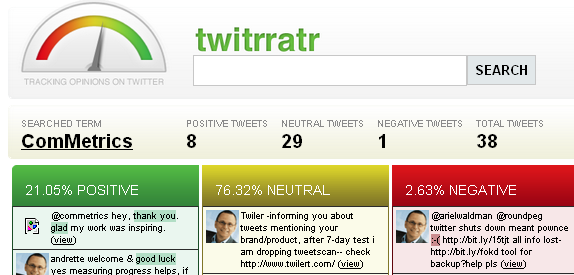
\includegraphics[scale = 0.4]{pics/tweetOpinions.png}
        \end{figure}
\end{itemize}
\end{scriptsize}

\end{frame}


\begin{frame}{Opinion Mining or Sentiment Analysis}
\begin{scriptsize}

\begin{block}{Twitter Sentiment Analysis Main Tasks}
\begin{enumerate}
\item  \textbf{Message-level polarity classification} (MPC): classify tweets into sentiment categories such as \textcolor[rgb]{0.00,0.00,1.00}{\textbf{positive}} and \textcolor[rgb]{1.00,0.00,0.00}{\textbf{negative}}.
\item \textbf{Polarity lexicon induction} (PLI): classify words from a corpus of tweets into sentiment categories, e.g.,  \textcolor[rgb]{0.00,0.00,1.00}{\textbf{happy, wonderful}}, \textcolor[rgb]{1.00,0.00,0.00}{\textbf{sad, bad}}.
\end{enumerate}
\end{block}

\begin{itemize}
\item  State-of-the-art solutions use \textbf{supervised} machine learning models trained from \textbf{manually} annotated examples.
\item \textbf{Problem}: annotation of words or tweets based on polarity classes is a \textbf{time-consuming} and \textbf{labor-intensive task}. 
\item \textbf{Possible Solution}: Transferring \textbf{existing labels} from a related problem domain.
\end{itemize}



 
\end{scriptsize}

\end{frame}





\begin{frame}{Transfer Learning Approach}
\begin{scriptsize}
\begin{itemize}
\item \textbf{Transfer learning}: improving learning task for a \textbf{target domain} $\mathcal{D_T}$ using knowledge obtained from a related \textbf{source domain} $\mathcal{D_S}$.
\item We transfer \textbf{sentiment knowledge} from the word domain  $\mathcal{D_W}$  to the message domain $\mathcal{D_M}$ and \textbf{vice versa}.
\item Tweets and words can be labelled according to the \textbf{same sentiment categories}, e.g, positive and negative ($\mathcal{Y_W}=\mathcal{Y_M}$).
\item We propose a \textbf{unified representation} that allows the bidirectional transfer of sentiment classifiers between words and tweets. 

\end{itemize}
\end{scriptsize}
\end{frame}


\begin{frame}{The word-tweet sentiment-interdependence relation}
\begin{scriptsize}
\begin{enumerate}
\item The polarity of a tweet is \textbf{determined} by the polarity of the words it \textbf{contains}.
\item The polarity of a word is \textbf{determined} by the polarity of the tweets in which it \textbf{occurs}. 
\end{enumerate}
\end{scriptsize}

\begin{figure}[htb]
\begin{center}
\scalebox{0.45}{
\begin{tabular}{cc}
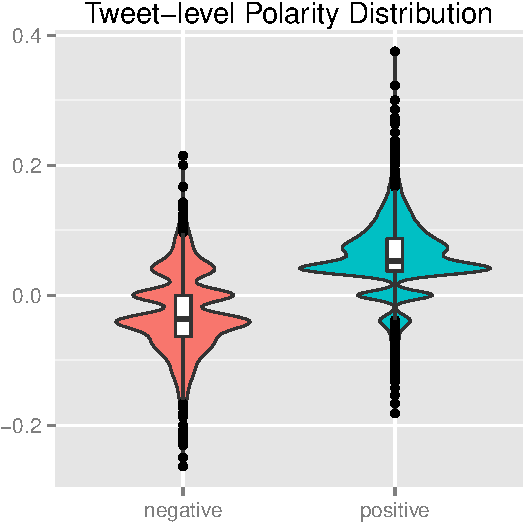
\includegraphics{pics/tweetPlotCrop.pdf} &  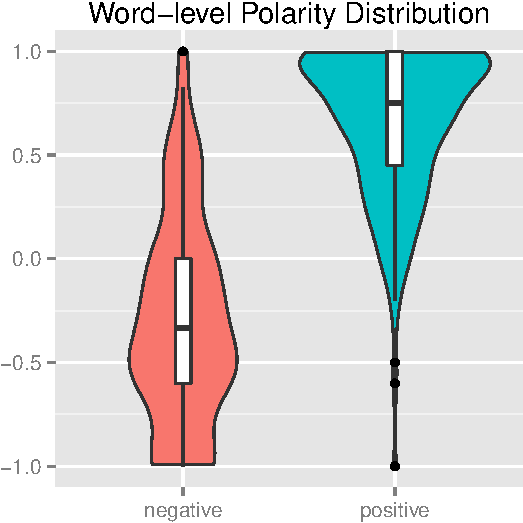
\includegraphics{pics/wordPlotPrun.pdf} 
\end{tabular}}
\caption{Violin plots of the polarity of tweets and words.}
\label{fig:vio}
\end{center}
\end{figure}

\end{frame} 


\begin{frame}{Transfer Learning with Tweet Centroids}
\begin{scriptsize}
\begin{itemize}
\item We represent tweets and words by \textbf{feature vectors} of the \textbf{same dimensionality}. 
\item Tweets are represented using \textbf{NLP features}: 1) unigrams, 2) part-of-speech (POS) tags, and 3) Brown words clusters.
\item \textbf{Tweet Centroid Model (TCM)}: words are represented by the \textbf{centroids} of the tweet vectors in which they \textbf{occur}.
\item TCM allows \textbf{classifiers} trained from one of the two domains to be \textbf{deployed} on data from the other.
\end{itemize}
\end{scriptsize}
\end{frame}





\begin{frame}{Transfer Learning with Tweet Centroids (2)}

\begin{figure}[htb]
	\centering
	 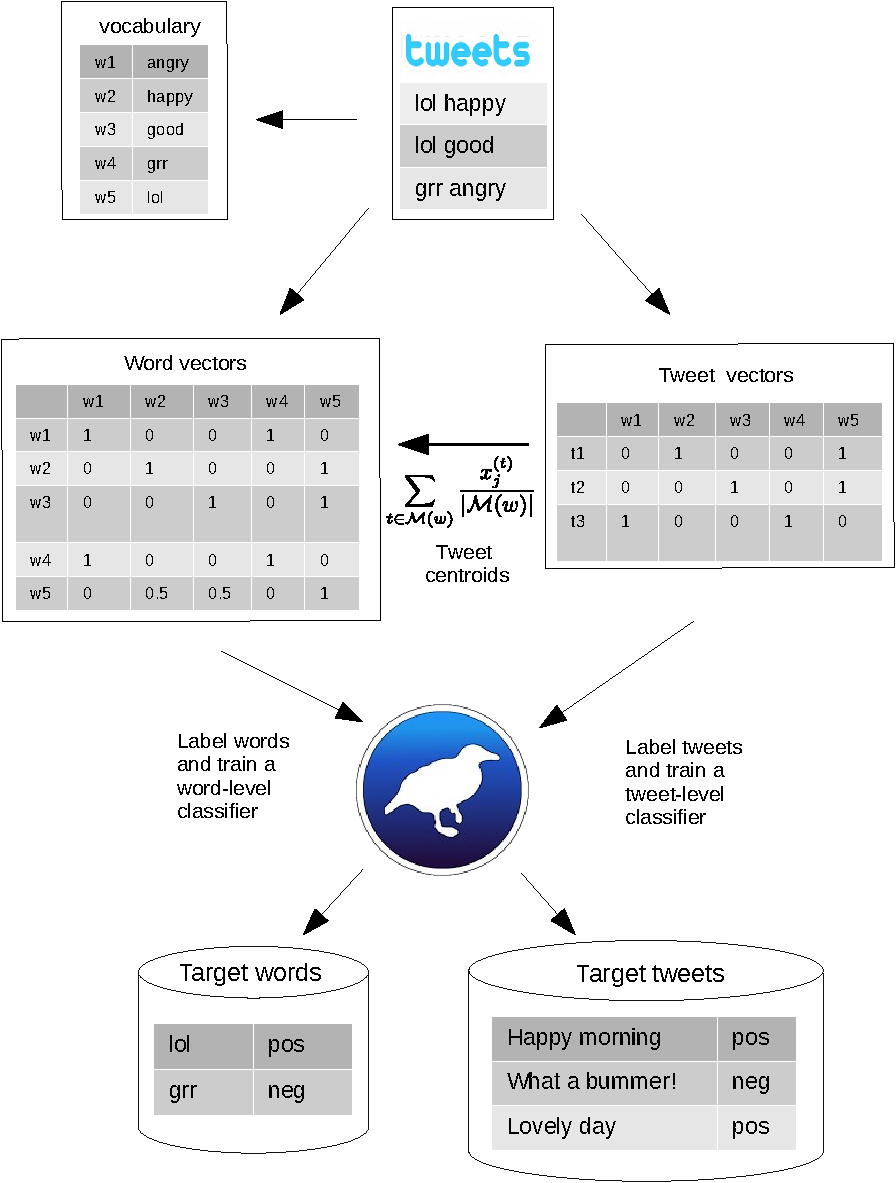
\includegraphics[scale=0.4]{pics/tweetsToWords.pdf}
\end{figure}



\end{frame}



\begin{frame}{Inducing a Lexicon from Labelled Tweets}
\begin{scriptsize}
\begin{itemize}
 \item We can train a \textbf{message-level classifier} $f_M$ from a corpus of sentiment annotated tweets $\mathcal{C}_L$ (SemEval) and deploy it on words found in a \textbf{corpus of unlabelled tweets} $\mathcal{C}_U$  represented by tweet centroids.
 \item We calculate the word-vectors from a \textbf{larger} corpus of unlabelled tweets (2M) to get \textbf{better} representations.
 \begin{table}[htbp]
\begin{tabular}{l|ll}
\hline \hline
\multicolumn{3}{c}{AUC} \\
\hline \hline
Source Dataset & PMI-SO & TCM  \\ \hline
Sanders & 0.757 &  \textbf{0.864} \\ 
6HumanCoded & 0.861 & \textbf{0.930}  \\ 
SemEval & 0.858 & \textbf{0.916}   \\ \hline
\end{tabular}
\caption{Word-level Polarity Classification Results for the AFINN lexicon.}
\end{table}
  \item TCM \textbf{outperformed} PMI-SO, a state-of-the-art measure for establishing world-level sentiment.
 \end{itemize}
\end{scriptsize}
\end{frame}



\begin{frame}{Inducing a Lexicon from Labelled Tweets}
\begin{figure}[htb]
\begin{center}
\scalebox{0.21}{
\begin{tabular}{cc}
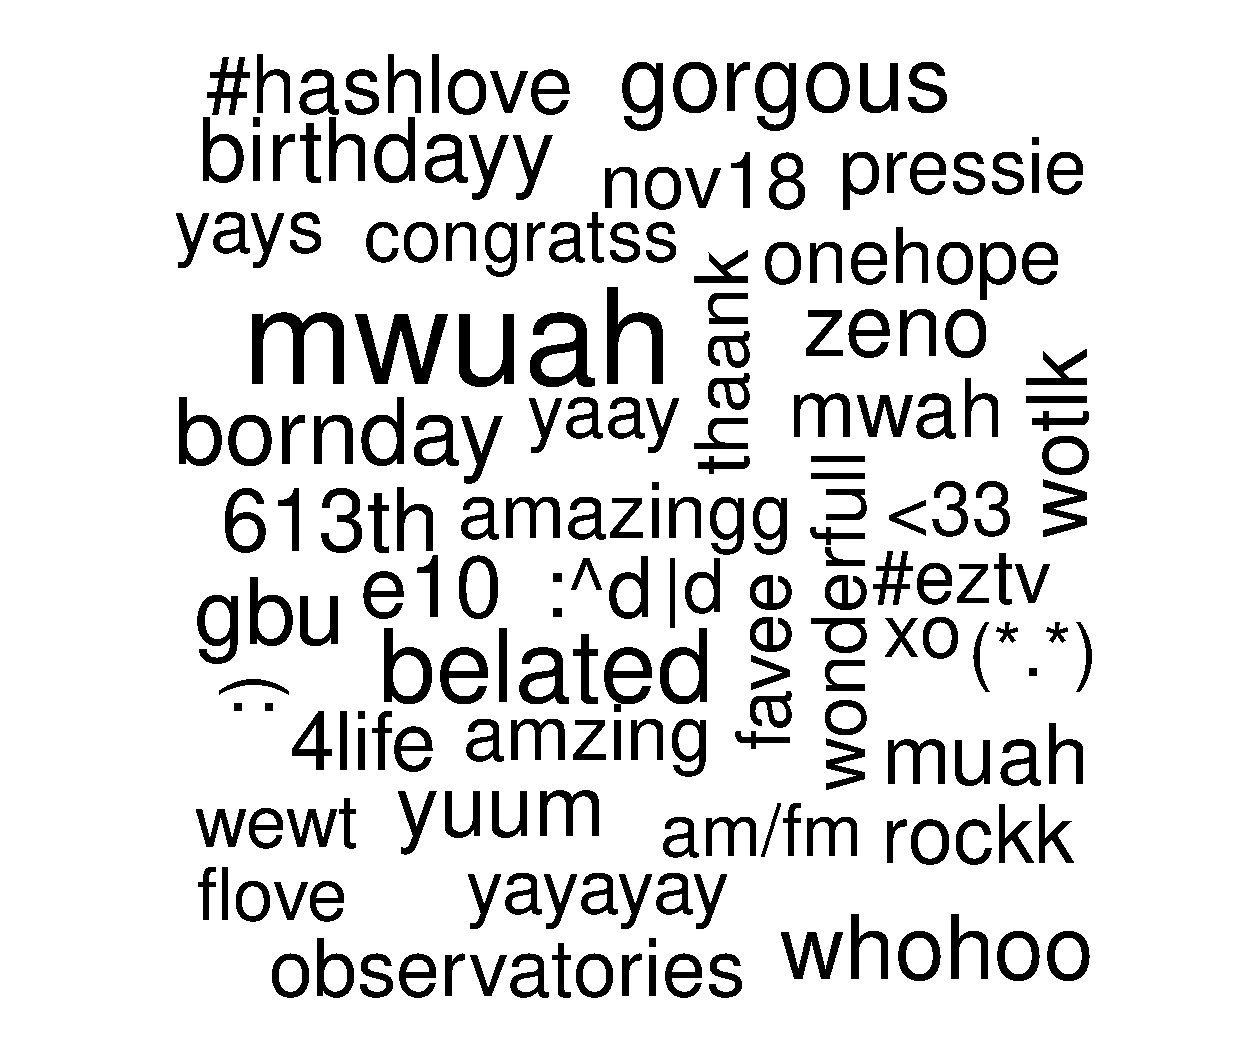
\includegraphics{pics/posWordsTranfer.pdf} & 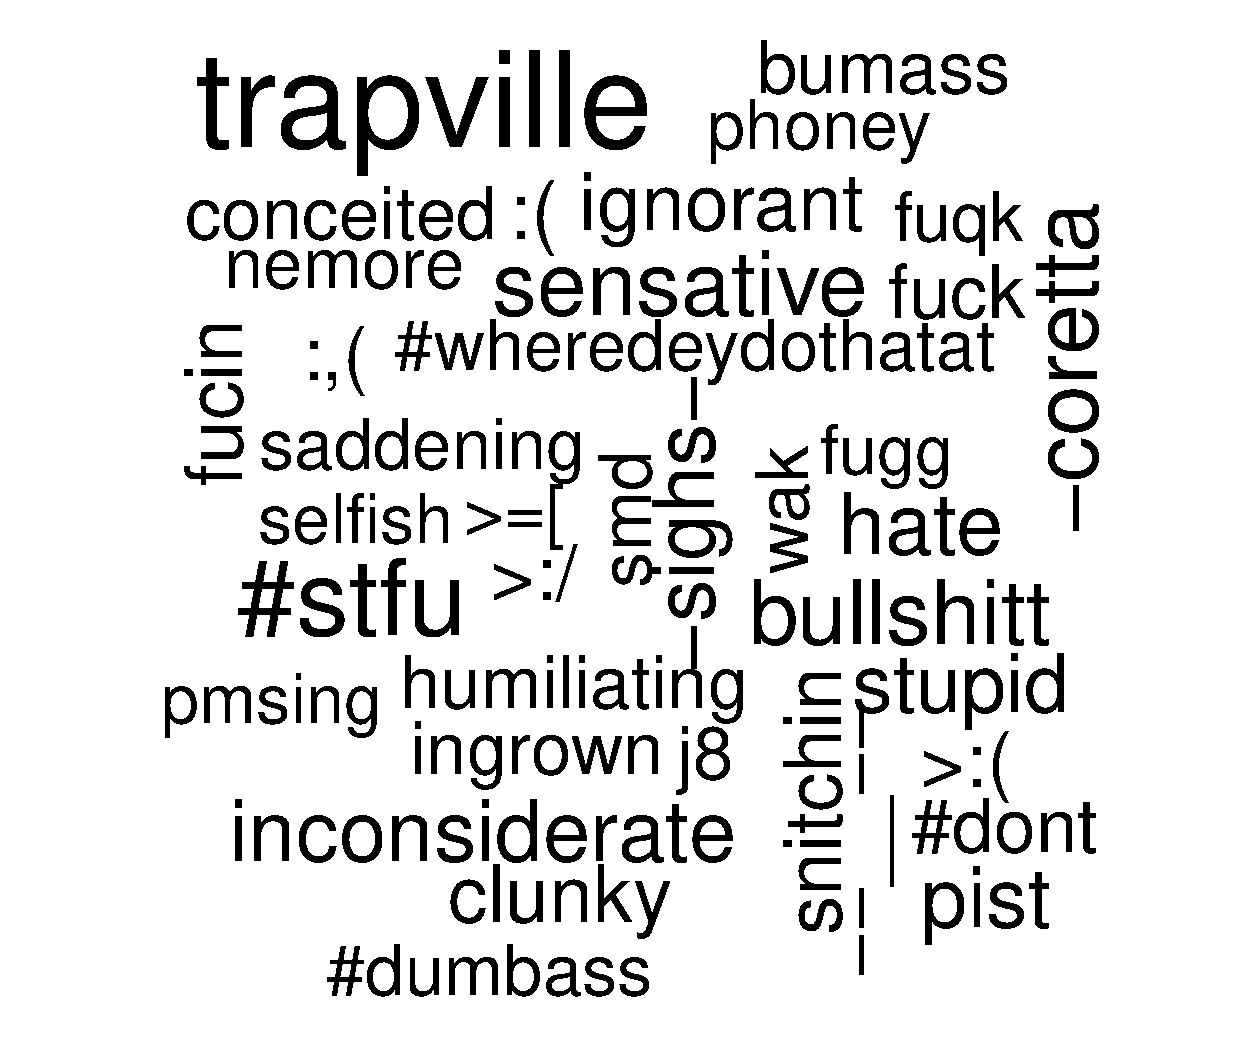
\includegraphics{pics/negWordsTranfer.pdf} \\
\end{tabular}}
\caption{Word clouds of positive and negative words obtained from a message-level classifier.}
\label{fig:wordcloud}
\end{center}
\end{figure}
\end{frame}

\begin{frame}{Tweet Centroids for message-level classification}
\begin{scriptsize}
\begin{itemize}
\item TCM can be used as a \textbf{distant supervision} model for MPC.
\item We use a \textbf{word-level} classifier $f_W$ trained with TCM vectors calculated from $\mathcal{C}_U$ labelled by a \textbf{polarity lexicon} $\mathcal{L}$. 
\item The classifier is deployed on the target tweets represented by \textbf{sparse vectors}.
\item The number of labelled words for training $f_W$ is \textbf{limited} to the number of words from $\mathcal{L}$.
\item TCM is \textbf{not capable} of exploiting large collections of unlabelled tweets for producing training datasets larger than the size of $\mathcal{L}$. 
\end{itemize}
\end{scriptsize}
\end{frame}

\begin{frame}{Partitioned TCM}
\begin{scriptsize}
\begin{itemize}
\item We propose a modification of our method for \textbf{increasing} the number labelled instances it produces. 
\item  The word-tweet set $\mathcal{M}(w)$ for each word from the lexicon ($w \in\mathcal{L}$) is \textbf{partitioned} into smaller disjoint subsets $\mathcal{M}(w)_1, \dots \mathcal{M}(w)_z$ of a fixed size determined by a parameter $p$. 
\item We calculate one tweet centroid vector $\overrightarrow{w}$ for \textbf{each partition} labelled according to $\mathcal{L}$.
\end{itemize}
\end{scriptsize}
\end{frame}


\begin{frame}{Baselines}
\begin{scriptsize}
\begin{block}{Emoticon-Annotation Approach (EAA)}
\begin{itemize}
\item Labels tweets with positive or negative emoticons according to the emoticon's polarity after removing the emoticon from the message.
\item  Tweets containing both positive and negative emoticons are \textbf{discarded}.
\end{itemize}
\end{block}

\begin{block}{Lexicon-annotation approach (LAA)}
\begin{itemize}
\item Uses a given polarity lexicon $\mathcal{L}$.
\item Tweets with at least one positive word and no negative word are labelled \textbf{positive}.
\item Tweets with at least one negative word and no positive word are labelled \textbf{negative}.
\end{itemize}
\end{block}

\end{scriptsize}
\end{frame}


\begin{frame}{Instances Generated by Distant Supervision Models}
We use 10 collections of 2 million tweets as source corpora.
\begin{table}
\begin{center}
\scalebox{0.7}{
\begin{tabular}{l|ll@{\hspace{0.1cm}}|ll@{\hspace{0.1cm}}|ll@{\hspace{0.1cm}}}
\hline
 & Avg. Positive & (\%) & Avg. Negative & (\%) & Avg. Total & (\%) \\ \hline
EAA & $130,641$ & (6.5\%) & $21,537$ & (1.1\%) & $152,179$ & (7.6\%) \\ 
LAA & $681,531$ & (34.1\%) & $294,177$ & (14.7\%) & $975,708$ & (48.8\%) \\ 
TCM & $1537$ & (0.05\%) & $951$ & (0.08\%) & $2488$ & (0.12\%) \\ 
TCM ($p$=5) & $276,696$ & (13.8\%) & $149,989$ & (7.5\%) & $426,684$ & (21.3\%) \\ 
TCM ($p$=10) & $138,596$ & (6.9\%) & $75,390$ & (3.8\%) & $213,986$ & (10.7\%) \\ 
TCM ($p$=20) & $69,518$  & (3.5\%) & $38,044$ & (1.9\%) & $107,563$ & (5.4\%) \\ 
TCM ($p$=50)& $32,231$ & (1.6\%) & $17,950$ & (0.9\%) & $50,181$ & (2.5\%) \\ 
TCM ($p$=100)& $14,338$ & (0.7\%) & $8357$ & (0.4\%) & $22,695$ & (1.1\%) \\ \hline
\end{tabular}}
\end{center}
\end{table} 


\end{frame}




\begin{frame}{TCM for MPC}

\begin{table}[htbp]
\begin{center}
\scalebox{0.8}{
\begin{tabular}{l|ll@{\hspace{0.1cm}}l@{\hspace{0.1cm}}|ll@{\hspace{0.1cm}}l@{\hspace{0.1cm}}|ll@{\hspace{0.1cm}}l@{\hspace{0.1cm}}}
\hline
 & \multicolumn{3}{c|}{6HumanCoded} & \multicolumn{3}{c|}{Sanders} & \multicolumn{3}{c}{SemEval} \\ \hline
EAA & 0.805 $\pm$ 0.005 & = & - & 0.800 $\pm$ 0.017 & = & +& 0.802  $\pm$ 0.006 & = & - \\ 
LAA & 0.809 $\pm$ 0.001 & + & = & 0.778 $\pm$ 0.002 & - & = & 0.814  $\pm$ 0.000 &+ & =\\ \hline
TCM & 0.776 $\pm$ 0.004 &-&-& 0.682 $\pm$ 0.024 &-&-& 0.779  $\pm$ 0.008 &-&-\\ 
TCM ($p$=5) & 0.834 $\pm$ 0.002 & + & +& 0.807 $\pm$ 0.008 &= & +& 0.833  $\pm$ 0.002 &+&+ \\ 
TCM ($p$=10) & 0.845 $\pm$ 0.003 & + & +& \textbf{0.817} $\pm$ 0.006 &+ & +& 0.841  $\pm$ 0.002 &+ & +\\ 
TCM ($p$=20) & \textbf{0.850} $\pm$ 0.003 &+ & +& 0.815 $\pm$ 0.011 &+ & +& \textbf{0.844}  $\pm$ 0.003 & + & +\\ 
TCM ($p$=50) & 0.844 $\pm$ 0.004 & + & +& 0.785 $\pm$ 0.010 & - & +& 0.836  $\pm$ 0.004 & + & +\\ 
TCM ($p$=100) & 0.829 $\pm$ 0.003 & + & +& 0.752 $\pm$ 0.019 & - & -& 0.821  $\pm$ 0.004 & + & +\\ \hline
\end{tabular}}
\end{center}
\caption{AUC for Message-level Polarity Classification. Best results per column are given in bold.}
\label{tab:messclas}
\end{table}
\end{frame}




\begin{frame}{Conclusions}
\begin{scriptsize}
\begin{itemize}
\item  We proposed a \textbf{distant supervision method} that outperformed LAA and EAA for MPC.

\item TCM is a \textbf{unified model} for message-level and word-level sentiment classification.


\item Future work: subjectivity, emotions, handle negations, non-linear representations and deep networks. 
\end{itemize}
\end{scriptsize}

\end{frame}

\begin{frame}
\frametitle{Questions?}
%\vspace{1.5cm}
\begin{center}\LARGE Thanks for your Attention!\\ \end{center}

\begin{columns}
\begin{column}{0.55\textwidth}
\begin{block}{Acknowledgements}
\begin{itemize}\tiny
	\item University of Waikato Doctoral Scholarship
	\item Machine Learning Group at the University of Waikato
	
\end{itemize}
\end{block}
\end{column}
\begin{column}{0.45\textwidth}
\vspace{1.5cm}

\begin{figure}[h!]
	\centering
	\includegraphics[scale=0.3]{../../img/waikato.png}
\end{figure}
\end{column}
\end{columns}

\end{frame}

\begin{frame}[allowframebreaks]\scriptsize
\frametitle{References}
\bibliography{../bio}
\bibliographystyle{apalike}
%\bibliographystyle{flexbib}
\end{frame}  


%%%%%%%%%%%%%%%%%%%%%%%%%%%

\end{document}
